\documentclass[aspectratio=169]{beamer}

% ============================================
% DATABRICKS THEME - COLOR DEFINITIONS
% ============================================
\usepackage{tikz}
\usepackage{graphicx}
\usepackage{hyperref}
\usepackage{xcolor}
\usepackage{booktabs}
\usepackage{fontspec}
\usepackage{listings}

% Databricks Color Palette
\definecolor{databricksBlue}{RGB}{41, 49, 66}
\definecolor{databricksRed}{RGB}{220, 53, 69}
\definecolor{databricksYellow}{RGB}{255, 193, 7}
\definecolor{databricksGreen}{RGB}{76, 175, 80}
\definecolor{databricksGray}{RGB}{128, 128, 128}
\definecolor{databricksLightGray}{RGB}{245, 245, 245}
\definecolor{databricksWhite}{RGB}{255, 255, 255}

% ============================================
% BEAMER THEME CONFIGURATION
% ============================================
\usetheme{default}
\usecolortheme{default}

% Set colors
\setbeamercolor{structure}{fg=databricksBlue}
\setbeamercolor{frametitle}{bg=databricksBlue, fg=databricksWhite}
\setbeamercolor{title}{fg=databricksWhite}
\setbeamercolor{subtitle}{fg=databricksLightGray}
\setbeamercolor{author}{fg=databricksWhite}
\setbeamercolor{date}{fg=databricksWhite}
\setbeamercolor{institute}{fg=databricksWhite}
\setbeamercolor{background canvas}{bg=databricksWhite}
\setbeamercolor{normal text}{fg=databricksBlue}
\setbeamercolor{itemize item}{fg=databricksBlue}
\setbeamercolor{itemize subitem}{fg=databricksRed}
\setbeamercolor{itemize subsubitem}{fg=databricksGreen}
\setbeamercolor{block title}{bg=databricksBlue, fg=databricksWhite}
\setbeamercolor{block body}{bg=databricksLightGray, fg=databricksBlue}

% Itemize symbols
\setbeamertemplate{itemize item}{\textcolor{databricksBlue}{$\bullet$}}
\setbeamertemplate{itemize subitem}{\textcolor{databricksRed}{$\triangleright$}}
\setbeamertemplate{itemize subsubitem}{\textcolor{databricksGreen}{$\circ$}}

% Remove navigation symbols
\setbeamertemplate{navigation symbols}{}

% ============================================
% CUSTOM FOOTER WITH HYPERLINKS
% ============================================
\setbeamertemplate{footline}{
    \leavevmode%
    \hbox{%
        \begin{beamercolorbox}[wd=.33\paperwidth,ht=2.5ex,dp=1ex,left]{author in head/foot}%
            \usebeamerfont{author in head/foot}\hspace*{2ex}%
            \href{https://easy-ai-labs.lovable.app/}{\textcolor{databricksBlue}{Easy AI Labs}}
        \end{beamercolorbox}%
        \begin{beamercolorbox}[wd=.34\paperwidth,ht=2.5ex,dp=1ex,center]{title in head/foot}%
            \usebeamerfont{title in head/foot}%
            \href{https://www.linkedin.com/in/yashkavaiya}{\textcolor{databricksBlue}{Yash Kavaiya}}
        \end{beamercolorbox}%
        \begin{beamercolorbox}[wd=.33\paperwidth,ht=2.5ex,dp=1ex,right]{date in head/foot}%
            \usebeamerfont{date in head/foot}%
            \href{https://www.linkedin.com/company/genai-guru}{\textcolor{databricksBlue}{Gen AI Guru}}\hspace*{2ex}
            \insertframenumber{} / \inserttotalframenumber\hspace*{2ex}
        \end{beamercolorbox}%
    }%
    \vskip0pt%
}

% ============================================
% TITLE PAGE CONFIGURATION
% ============================================
\setbeamertemplate{title page}{
    \begin{tikzpicture}[remember picture,overlay]
        \fill[databricksBlue] (current page.north west) rectangle (current page.south east);
    \end{tikzpicture}
    \vfill
    \begin{center}
        {\Huge\bfseries\textcolor{databricksWhite}{\inserttitle}\par}
        \vspace{0.5cm}
        {\large\textcolor{databricksYellow}{\insertsubtitle}\par}
        \vspace{1cm}
        {\textcolor{databricksWhite}{\insertauthor}\par}
        \vspace{0.3cm}
        {\small\textcolor{databricksLightGray}{\insertdate}\par}
    \end{center}
    \vfill
}

% ============================================
% DOCUMENT INFO
% ============================================
\title{Databricks Fundamentals}
\subtitle{Complete Guide to Modern Data Analytics}
\author{Yash Kavaiya}
\date{14-Day AI Challenge - Day 1}

\begin{document}

% ============================================
% TITLE SLIDE
% ============================================
\frame{\titlepage}

% ============================================
% TABLE OF CONTENTS
% ============================================
\begin{frame}{Agenda}
    \begin{columns}[T]
        \begin{column}{0.5\textwidth}
            \begin{itemize}
                \item \textcolor{databricksBlue}{\textbf{Introduction to Databricks}}
                \item \textcolor{databricksBlue}{\textbf{Why Databricks?}}
                    \begin{itemize}
                        \item Pandas vs Hadoop vs Spark
                        \item Evolution of Big Data
                    \end{itemize}
                \item \textcolor{databricksBlue}{\textbf{Lakehouse Architecture}}
                    \begin{itemize}
                        \item Data Warehouse vs Data Lake
                        \item Delta Lake Foundation
                    \end{itemize}
            \end{itemize}
        \end{column}
        \begin{column}{0.5\textwidth}
            \begin{itemize}
                \item \textcolor{databricksBlue}{\textbf{Workspace Structure}}
                    \begin{itemize}
                        \item Navigation \& Components
                        \item Compute Resources
                    \end{itemize}
                \item \textcolor{databricksBlue}{\textbf{Industry Use Cases}}
                    \begin{itemize}
                        \item Netflix, Shell, Comcast
                    \end{itemize}
                \item \textcolor{databricksBlue}{\textbf{Hands-On Tasks}}
            \end{itemize}
        \end{column}
    \end{columns}
\end{frame}

% ============================================
% SECTION 1: INTRODUCTION
% ============================================
\begin{frame}{What is Databricks?}
    \begin{block}{Definition}
        A \textbf{unified analytics platform} built on Apache Spark, providing a collaborative environment for data engineering, data science, and ML workloads.
    \end{block}
    \vspace{0.5cm}
    \begin{columns}[T]
        \begin{column}{0.5\textwidth}
            \textcolor{databricksBlue}{\textbf{Key Value Propositions:}}
            \begin{itemize}
                \item Unified platform for all data needs
                \item Built on open-source technologies
                \item Cloud-native (AWS, Azure, GCP)
                \item Collaborative notebooks
                \item Enterprise-grade security
            \end{itemize}
        \end{column}
        \begin{column}{0.5\textwidth}
            \textcolor{databricksRed}{\textbf{Founded by:}}
            \begin{itemize}
                \item Original creators of Apache Spark
                \item Creators of Delta Lake
                \item Creators of MLflow
                \item From UC Berkeley's AMPLab
            \end{itemize}
        \end{column}
    \end{columns}
\end{frame}

% ============================================
% SECTION 2: EVOLUTION OF BIG DATA
% ============================================
\begin{frame}{The Evolution of Big Data Processing}
    \begin{center}
        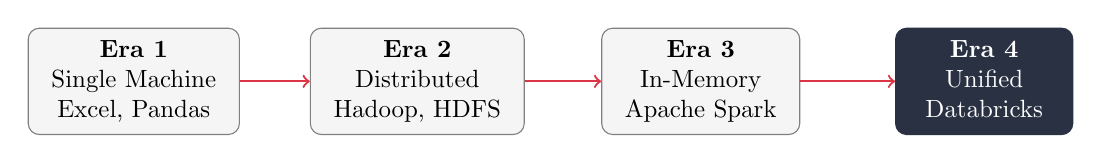
\begin{tikzpicture}[scale=0.9, every node/.style={transform shape}]
            % Era boxes
            \node[draw=databricksGray, fill=databricksLightGray, rounded corners, minimum width=2.5cm, minimum height=1.5cm] (era1) at (0,0) {\begin{tabular}{c}\textbf{Era 1}\\Single Machine\\Excel, Pandas\end{tabular}};
            
            \node[draw=databricksGray, fill=databricksLightGray, rounded corners, minimum width=2.5cm, minimum height=1.5cm] (era2) at (4,0) {\begin{tabular}{c}\textbf{Era 2}\\Distributed\\Hadoop, HDFS\end{tabular}};
            
            \node[draw=databricksGray, fill=databricksLightGray, rounded corners, minimum width=2.5cm, minimum height=1.5cm] (era3) at (8,0) {\begin{tabular}{c}\textbf{Era 3}\\In-Memory\\Apache Spark\end{tabular}};
            
            \node[draw=databricksBlue, fill=databricksBlue, text=databricksWhite, rounded corners, minimum width=2.5cm, minimum height=1.5cm] (era4) at (12,0) {\begin{tabular}{c}\textbf{Era 4}\\Unified\\Databricks\end{tabular}};
            
            % Arrows
            \draw[->, thick, databricksRed] (era1) -- (era2);
            \draw[->, thick, databricksRed] (era2) -- (era3);
            \draw[->, thick, databricksRed] (era3) -- (era4);
        \end{tikzpicture}
    \end{center}
    \vspace{0.5cm}
    \begin{alertblock}{Key Insight}
        Each era solved specific problems but introduced new challenges, leading to the next evolution.
    \end{alertblock}
\end{frame}

% ============================================
% PANDAS LIMITATIONS
% ============================================
\begin{frame}{Pandas: Strengths \& Limitations}
    \begin{columns}[T]
        \begin{column}{0.5\textwidth}
            \textcolor{databricksGreen}{\textbf{Strengths:}}
            \begin{itemize}
                \item Intuitive API with rich functionality
                \item Fast for small datasets (< few GB)
                \item Extensive ecosystem support
                \item Great for exploratory analysis
                \item Excellent visualization integration
            \end{itemize}
        \end{column}
        \begin{column}{0.5\textwidth}
            \textcolor{databricksRed}{\textbf{Limitations:}}
            \begin{itemize}
                \item \textbf{Memory Bound:} Data must fit in RAM
                \item \textbf{Single Machine:} No distribution
                \item \textbf{Vertical Scaling Only}
                \item \textbf{No Lazy Evaluation}
                \item \textbf{Limited Fault Tolerance}
            \end{itemize}
        \end{column}
    \end{columns}
    \vspace{0.5cm}
    \begin{block}{The Memory Problem}
        If you have a 10GB CSV and 8GB RAM: \textcolor{databricksRed}{\textbf{Pandas fails!}}\\
        Actual memory needed $\approx$ Data Size $\times$ 2 to 5x (due to intermediate copies)
    \end{block}
\end{frame}

% ============================================
% HADOOP LIMITATIONS
% ============================================
\begin{frame}{Hadoop: The Original Big Data Solution}
    \begin{columns}[T]
        \begin{column}{0.5\textwidth}
            \textcolor{databricksBlue}{\textbf{Components:}}
            \begin{itemize}
                \item \textbf{HDFS:} Distributed File System
                \item \textbf{MapReduce:} Processing Model
                \item \textbf{YARN:} Resource Management
                \item \textbf{Hive, Pig, HBase:} Tools
            \end{itemize}
        \end{column}
        \begin{column}{0.5\textwidth}
            \textcolor{databricksRed}{\textbf{Limitations:}}
            \begin{itemize}
                \item Disk-Based (10-100x slower)
                \item High Latency (minutes/job)
                \item Complex MapReduce code
                \item Batch only, no streaming
                \item Multiple tools required
            \end{itemize}
        \end{column}
    \end{columns}
    \vspace{0.5cm}
    \begin{alertblock}{The I/O Bottleneck}
        Every operation involves disk read/write. For iterative ML algorithms:\\
        Time = n $\times$ (Disk Read + Disk Write) $\Rightarrow$ \textbf{Prohibitively slow!}
    \end{alertblock}
\end{frame}

% ============================================
% APACHE SPARK
% ============================================
\begin{frame}{Apache Spark: The Game Changer}
    \begin{block}{Core Innovation: In-Memory Computing}
        \textbf{RDDs} (Resilient Distributed Datasets) - \textbf{Resilient, Distributed, Parallel}
    \end{block}
    \vspace{0.3cm}
    \begin{columns}[T]
        \begin{column}{0.5\textwidth}
            \textcolor{databricksBlue}{\textbf{Spark Unified Stack:}}
            \begin{itemize}
                \item \textbf{Spark SQL:} Structured data
                \item \textbf{Spark Streaming:} Real-time
                \item \textbf{MLlib:} Machine Learning
                \item \textbf{GraphX:} Graph processing
            \end{itemize}
        \end{column}
        \begin{column}{0.5\textwidth}
            \textcolor{databricksGreen}{\textbf{Performance:}}
            \begin{itemize}
                \item \textbf{100x} faster than Hadoop (in-memory)
                \item \textbf{10x} faster (on-disk)
                \item Memory: 100 nanoseconds
                \item Disk: 10 milliseconds
            \end{itemize}
        \end{column}
    \end{columns}
    \vspace{0.3cm}
    \begin{center}
        \textcolor{databricksRed}{\textbf{Hadoop:}} Read $\rightarrow$ Process $\rightarrow$ Write $\rightarrow$ Read $\rightarrow$ Process $\rightarrow$ Write\\
        \textcolor{databricksGreen}{\textbf{Spark:}} Read $\rightarrow$ Process $\rightarrow$ Process $\rightarrow$ Process $\rightarrow$ Write (final only)
    \end{center}
\end{frame}

% ============================================
% DATABRICKS VALUE ADD
% ============================================
\begin{frame}{Databricks: Beyond Open-Source Spark}
    \begin{center}
        \textit{``While Spark is the engine, Databricks is the complete vehicle''}
    \end{center}
    \vspace{0.3cm}
    \begin{columns}[T]
        \begin{column}{0.5\textwidth}
            \textcolor{databricksBlue}{\textbf{Open-Source Spark:}}
            \begin{itemize}
                \item Manual cluster configuration
                \item Base Spark speed
                \item Jupyter (separate)
                \item External scheduling tools
                \item Self-managed Delta Lake
            \end{itemize}
        \end{column}
        \begin{column}{0.5\textwidth}
            \textcolor{databricksGreen}{\textbf{Databricks Platform:}}
            \begin{itemize}
                \item \textbf{One-click clusters}
                \item \textbf{2-5x faster} with Photon
                \item \textbf{Integrated notebooks}
                \item \textbf{Built-in Workflows}
                \item \textbf{Unity Catalog governance}
            \end{itemize}
        \end{column}
    \end{columns}
    \vspace{0.3cm}
    \begin{block}{Databricks Runtime (DBR)}
        Pre-installed libraries $\bullet$ Photon engine (C++, 2-8x faster) $\bullet$ GPU support $\bullet$ Optimized I/O
    \end{block}
\end{frame}

% ============================================
% COMPARISON TABLE
% ============================================
\begin{frame}{Comprehensive Comparison}
    \begin{center}
        \scriptsize
        \begin{tabular}{l|cccc}
            \toprule
            \textbf{Criteria} & \textbf{Pandas} & \textbf{Hadoop} & \textbf{Spark} & \textbf{Databricks} \\
            \midrule
            Data Size & MB-GB & TB-PB & TB-PB & TB-PB \\
            Processing & Single & Distributed (disk) & Distributed (mem) & Optimized \\
            Speed & Fast (small) & Slow & 100x Hadoop & 2-5x Spark \\
            Real-time & No & No & Yes & Yes (enhanced) \\
            ML Support & scikit-learn & Mahout & MLlib & MLlib + MLflow \\
            Governance & Manual & Limited & Limited & \textcolor{databricksGreen}{\textbf{Unity Catalog}} \\
            \bottomrule
        \end{tabular}
    \end{center}
    \vspace{0.5cm}
    \begin{block}{Decision Guide}
        \textbf{< 10GB:} Pandas $\bullet$ \textbf{10GB-1TB + Collaboration:} Databricks $\bullet$ \textbf{> 1TB + Enterprise:} Databricks
    \end{block}
\end{frame}

% ============================================
% LAKEHOUSE ARCHITECTURE
% ============================================
\begin{frame}{Data Architecture Evolution}
    \begin{columns}[T]
        \begin{column}{0.5\textwidth}
            \textcolor{databricksBlue}{\textbf{Data Warehouse (1980s-2000s):}}
            \begin{itemize}
                \item Structured data only
                \item ACID transactions
                \item SQL-based
                \item High cost/TB
                \item No unstructured data
            \end{itemize}
            \vspace{0.3cm}
            \textcolor{databricksRed}{\textbf{Data Lake (2010s):}}
            \begin{itemize}
                \item All data types
                \item Schema-on-read
                \item Low cost storage
                \item Poor reliability
                \item ``Data Swamps''
            \end{itemize}
        \end{column}
        \begin{column}{0.5\textwidth}
            \begin{block}{The Two-Tier Problem}
                Organizations ended up with \textbf{BOTH}:\\
                $\Rightarrow$ Data duplication\\
                $\Rightarrow$ Stale data\\
                $\Rightarrow$ Complex pipelines\\
                $\Rightarrow$ High costs\\
                $\Rightarrow$ Governance challenges
            \end{block}
            \vspace{0.3cm}
            \begin{alertblock}{Solution}
                \textcolor{databricksGreen}{\textbf{Data Lakehouse!}}
            \end{alertblock}
        \end{column}
    \end{columns}
\end{frame}

% ============================================
% LAKEHOUSE DEFINITION
% ============================================
\begin{frame}{What is a Data Lakehouse?}
    \begin{block}{Definition}
        \textbf{Lakehouse} = Data Lake (flexibility, low cost) + Data Warehouse (reliability, governance)
    \end{block}
    \vspace{0.3cm}
    \begin{columns}[T]
        \begin{column}{0.5\textwidth}
            \textcolor{databricksBlue}{\textbf{Key Principles:}}
            \begin{itemize}
                \item \textbf{Open Formats:} Parquet, Delta
                \item \textbf{ACID Transactions}
                \item \textbf{Schema Enforcement}
                \item \textbf{Time Travel}
                \item \textbf{Unified Access}
                \item \textbf{Direct Access}
            \end{itemize}
        \end{column}
        \begin{column}{0.5\textwidth}
            \textcolor{databricksGreen}{\textbf{Benefits:}}
            \begin{itemize}
                \item No vendor lock-in
                \item Data consistency
                \item Prevent bad data
                \item Auditing \& rollback
                \item No data silos
                \item No data copying
            \end{itemize}
        \end{column}
    \end{columns}
    \vspace{0.3cm}
    \begin{center}
        \textbf{One platform $\rightarrow$ All workloads:} BI, Data Science, ML, Streaming
    \end{center}
\end{frame}

% ============================================
% DELTA LAKE
% ============================================
\begin{frame}{Delta Lake: The Foundation}
    \begin{block}{What is Delta Lake?}
        An open-source storage layer that brings \textbf{reliability} to Data Lakes.
    \end{block}
    \vspace{0.3cm}
    \begin{columns}[T]
        \begin{column}{0.5\textwidth}
            \textcolor{databricksBlue}{\textbf{How It Works:}}
            \begin{itemize}
                \item Parquet files + Transaction Log
                \item Each operation logged in JSON
                \item Enables version tracking
                \item Atomic commits
            \end{itemize}
        \end{column}
        \begin{column}{0.5\textwidth}
            \textcolor{databricksGreen}{\textbf{Key Features:}}
            \begin{itemize}
                \item \textbf{ACID Transactions}
                \item \textbf{Time Travel}
                \item \textbf{Schema Evolution}
                \item \textbf{Audit History}
                \item \textbf{MERGE (Upserts)}
                \item \textbf{Optimize \& Z-Order}
            \end{itemize}
        \end{column}
    \end{columns}
    \vspace{0.3cm}
    \begin{exampleblock}{Time Travel Example}
        \texttt{SELECT * FROM sales VERSION AS OF 5;}\\
        \texttt{RESTORE TABLE sales TO VERSION AS OF 5;}
    \end{exampleblock}
\end{frame}

% ============================================
% MEDALLION ARCHITECTURE
% ============================================
\begin{frame}{Medallion Architecture}
    \begin{center}
        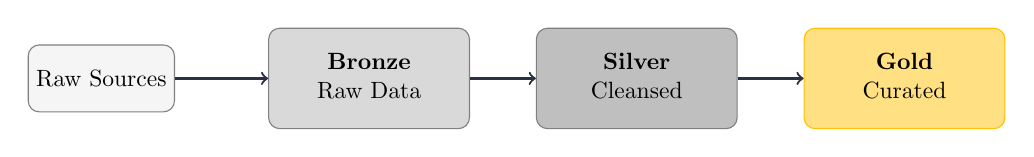
\begin{tikzpicture}[scale=0.85, every node/.style={transform shape}]
            % Sources
            \node[draw=databricksGray, fill=databricksLightGray, rounded corners, minimum width=2cm, minimum height=1cm] (src) at (0,0) {Raw Sources};
            
            % Bronze
            \node[draw=databricksGray, fill=databricksGray!30, rounded corners, minimum width=3cm, minimum height=1.5cm] (bronze) at (4,0) {\begin{tabular}{c}\textbf{Bronze}\\Raw Data\end{tabular}};
            
            % Silver
            \node[draw=databricksGray, fill=databricksGray!50, rounded corners, minimum width=3cm, minimum height=1.5cm] (silver) at (8,0) {\begin{tabular}{c}\textbf{Silver}\\Cleansed\end{tabular}};
            
            % Gold
            \node[draw=databricksYellow, fill=databricksYellow!50, rounded corners, minimum width=3cm, minimum height=1.5cm] (gold) at (12,0) {\begin{tabular}{c}\textbf{Gold}\\Curated\end{tabular}};
            
            % Arrows
            \draw[->, thick, databricksBlue] (src) -- (bronze);
            \draw[->, thick, databricksBlue] (bronze) -- (silver);
            \draw[->, thick, databricksBlue] (silver) -- (gold);
        \end{tikzpicture}
    \end{center}
    \vspace{0.3cm}
    \scriptsize
    \begin{tabular}{l|lll}
        \toprule
        & \textbf{Bronze} & \textbf{Silver} & \textbf{Gold} \\
        \midrule
        Purpose & Store raw data & Clean \& validate & Business aggregates \\
        Quality & Low (errors, dupes) & Medium (rules applied) & High (analytics ready) \\
        Schema & Schema-on-read & Schema enforced & Denormalized \\
        \bottomrule
    \end{tabular}
\end{frame}

% ============================================
% WORKSPACE STRUCTURE
% ============================================
\begin{frame}{Databricks Workspace Structure}
    \begin{columns}[T]
        \begin{column}{0.5\textwidth}
            \textcolor{databricksBlue}{\textbf{Main Navigation:}}
            \begin{itemize}
                \item \textbf{Home:} Personal workspace
                \item \textbf{Workspace:} Shared folders
                \item \textbf{Repos:} Git integration
                \item \textbf{Catalog:} Unity Catalog
                \item \textbf{Workflows:} Job orchestration
                \item \textbf{Compute:} Clusters, Warehouses
                \item \textbf{ML:} Experiments, Models
            \end{itemize}
        \end{column}
        \begin{column}{0.5\textwidth}
            \textcolor{databricksGreen}{\textbf{Compute Types:}}
            \begin{itemize}
                \item \textbf{All-Purpose Cluster:} Development
                \item \textbf{Job Cluster:} Production jobs
                \item \textbf{SQL Warehouse:} SQL analytics
                \item \textbf{Instance Pool:} Pre-warmed
            \end{itemize}
            \vspace{0.3cm}
            \textcolor{databricksRed}{\textbf{Runtimes:}}
            \begin{itemize}
                \item Standard, ML, Photon, GPU
            \end{itemize}
        \end{column}
    \end{columns}
\end{frame}

% ============================================
% NOTEBOOKS
% ============================================
\begin{frame}{Databricks Notebooks}
    \begin{block}{Interactive documents for code, visualizations, and narrative text}
    \end{block}
    \vspace{0.3cm}
    \begin{columns}[T]
        \begin{column}{0.5\textwidth}
            \textcolor{databricksBlue}{\textbf{Supported Languages:}}
            \begin{itemize}
                \item \texttt{\%python} - Default
                \item \texttt{\%sql} - Data queries
                \item \texttt{\%scala} - Performance
                \item \texttt{\%r} - Statistics
                \item \texttt{\%md} - Documentation
                \item \texttt{\%sh} - Shell commands
            \end{itemize}
        \end{column}
        \begin{column}{0.5\textwidth}
            \textcolor{databricksGreen}{\textbf{Key Features:}}
            \begin{itemize}
                \item Built-in Visualizations
                \item Dashboard Widgets
                \item Real-time Collaboration
                \item Revision History
                \item Interactive Parameters
            \end{itemize}
        \end{column}
    \end{columns}
    \vspace{0.3cm}
    \begin{exampleblock}{Widget Example}
        \texttt{dbutils.widgets.dropdown("region", "US", ["US", "EU", "APAC"])}
    \end{exampleblock}
\end{frame}

% ============================================
% USE CASE: NETFLIX
% ============================================
\begin{frame}{Industry Use Case: Netflix}
    \begin{block}{The Challenge}
        230+ million subscribers $\bullet$ 1+ billion hours/week $\bullet$ Real-time personalization
    \end{block}
    \vspace{0.3cm}
    \begin{columns}[T]
        \begin{column}{0.5\textwidth}
            \textcolor{databricksBlue}{\textbf{Implementation:}}
            \begin{itemize}
                \item Real-time Recommendations
                \item A/B Testing Platform
                \item Content Analytics
                \item Stream Quality Monitoring
            \end{itemize}
        \end{column}
        \begin{column}{0.5\textwidth}
            \textcolor{databricksGreen}{\textbf{Scale:}}
            \begin{itemize}
                \item \textbf{1.5 trillion} events/day
                \item \textbf{100+ PB} in data lake
                \item Updates every \textbf{10 seconds}
                \item \textbf{1000s} of A/B tests
            \end{itemize}
        \end{column}
    \end{columns}
    \vspace{0.3cm}
    \begin{center}
        \textbf{Tech Stack:} Kafka $\rightarrow$ Spark Streaming $\rightarrow$ Delta Lake $\rightarrow$ ML Models
    \end{center}
\end{frame}

% ============================================
% HANDS-ON TASKS
% ============================================
\begin{frame}{Hands-On Tasks}
    \begin{enumerate}
        \item \textcolor{databricksBlue}{\textbf{Create Databricks Community Edition Account}}
            \begin{itemize}
                \item Visit \href{https://community.cloud.databricks.com}{community.cloud.databricks.com}
                \item Sign up with email
            \end{itemize}
        \vspace{0.3cm}
        \item \textcolor{databricksBlue}{\textbf{Navigate Workspace, Compute, Data Explorer}}
            \begin{itemize}
                \item Explore left navigation panel
                \item Create a cluster
            \end{itemize}
        \vspace{0.3cm}
        \item \textcolor{databricksBlue}{\textbf{Create Your First Notebook}}
            \begin{itemize}
                \item New $\rightarrow$ Notebook
                \item Attach to cluster
            \end{itemize}
        \vspace{0.3cm}
        \item \textcolor{databricksBlue}{\textbf{Run Basic PySpark Commands}}
            \begin{itemize}
                \item \texttt{spark.range(10).show()}
            \end{itemize}
    \end{enumerate}
\end{frame}

% ============================================
% KEY TAKEAWAYS
% ============================================
\begin{frame}{Key Takeaways}
    \begin{columns}[T]
        \begin{column}{0.5\textwidth}
            \begin{block}{Remember}
                \begin{itemize}
                    \item Databricks = Unified Analytics Platform
                    \item Lakehouse = Lake + Warehouse benefits
                    \item Delta Lake = ACID + Time Travel
                    \item Medallion = Bronze $\rightarrow$ Silver $\rightarrow$ Gold
                \end{itemize}
            \end{block}
        \end{column}
        \begin{column}{0.5\textwidth}
            \begin{alertblock}{Why Databricks?}
                \begin{itemize}
                    \item \textbf{100x} faster than Hadoop
                    \item \textbf{2-5x} faster than Spark
                    \item \textbf{Unified} governance
                    \item \textbf{Collaborative} notebooks
                \end{itemize}
            \end{alertblock}
        \end{column}
    \end{columns}
    \vspace{0.5cm}
    \begin{center}
        \Large\textcolor{databricksBlue}{\textbf{Start your Databricks journey today!}}
    \end{center}
\end{frame}

% ============================================
% THANK YOU SLIDE
% ============================================
\begin{frame}
    \begin{tikzpicture}[remember picture,overlay]
        \fill[databricksBlue] (current page.north west) rectangle (current page.south east);
    \end{tikzpicture}
    \begin{center}
        \vspace{2cm}
        {\Huge\bfseries\textcolor{databricksWhite}{Thank You!}\par}
        \vspace{1cm}
        {\large\textcolor{databricksYellow}{Questions?}\par}
        \vspace{1.5cm}
        {\textcolor{databricksWhite}{Connect with me:}\par}
        \vspace{0.3cm}
        {\href{https://www.linkedin.com/in/yashkavaiya}{\textcolor{databricksLightGray}{linkedin.com/in/yashkavaiya}}\par}
        \vspace{0.3cm}
        {\href{https://www.linkedin.com/company/genai-guru}{\textcolor{databricksLightGray}{Gen AI Guru}}\par}
    \end{center}
\end{frame}

\end{document}
